\chapter{Design}
\label{sec:design}

% Ist das zentrale Kapitel der Arbeit. Hier werden das Ziel sowie die
% eigenen Ideen, Wertungen, Entwurfsentscheidungen vorgebracht. Es kann
% sich lohnen, verschiedene Möglichkeiten durchzuspielen und dann
% explizit zu begründen, warum man sich für eine bestimmte entschieden
% hat. Dieses Kapitel sollte - zumindest in Stichworten - schon bei den
% ersten Festlegungen eines Entwurfs skizziert werden.
% Es wird sich aber in einer normal verlaufenden
% Arbeit dauernd etwas daran ändern. Das Kapitel darf nicht zu
% detailliert werden, sonst langweilt sich der Leser. Es ist sehr
% wichtig, das richtige Abstraktionsniveau zu finden. Beim Verfassen
% sollte man auf die Wiederverwendbarkeit des Textes achten.

% Plant man eine Veröffentlichung aus der Arbeit zu machen, können von
% diesem Kapitel Teile genommen werden. Das Kapitel wird in der Regel
% wohl mindestens 8 Seiten haben, mehr als 20 können ein Hinweis darauf
% sein, daß das Abstraktionsniveau verfehlt wurde.

%\ldots design \ldots

%\todo{write design}
This chapter presents a design proposal for a shielding interface that protects applications from being compromised by the OCI interface. Our discussion revolves around the design's various components, functions, interactions, and security 
implications. Our proposed design includes the following parts:

\textbf{Remote attestation and secret provisioning Infrastructure.} This infrastructure forms the cornerstone of secure application deployment and operation by ensuring proper application launch and safeguarding the integrity and confidentiality of 
secrets provisioned by the application owner. Secrets management and deployment are offloaded from Kubernetes and Quark Shim to a trusted relying party. The shield relies on this infrastructure to measure the application launch process and 
establish secure communication with the relying party for secret retrieval.

\textbf{A new pattern for EXEC requests.} This pattern is designed to address three security concerns, namely issuing unauthorized commands to the application, unrestricted allocation of a terminal using kubectl exec -it, and lack of protection for 
commands issued by the application owner. We will explain this further in Section 3.2.
 

\textbf{A mechanism for protecting guest processes' stdio.} This mechanism ensures the protection of the confidentiality and integrity of application logs and terminal data streams belonging to the application owner and prevents attackers from stealing 
the execution results of privileged commands.

\textbf{System call interception.} A user-configurable guest system call interception policy.

\textbf{Qkenrell Log management.} A user-configurable guest logging protection policy.

In the following sections, we first describe the remote attestation and provisioning infrastructure in Section 4.1. We then introduce the new pattern of EXEC requests, the mechanism for protecting the standard IO of guest processes, the guest 
system call interceptor, and the guest log management policy in Sections 4.2, 4.3, 4.4, and 4.5, respectively. Finally, we propose modifications to the OCI interface in Section 4.6.


\section{General Architecture}
The secure virtual machine provides a trusted execution environment that encapsulates the guest, including the Qkernel and application. This environment is also known as an enclave. However, since the Qkernel uses the Qcall, Ucall, and Hcall 
interface to access host services, the shielding layer is added to the Qkernel to prevent attackers from exploiting these interfaces to launch attacks on the enclave. The shield layer controls the communication between the Qkernel and untrusted 
hosts via Ucall, Qcall, and Hcall, modifying the communication according to the shield policy set by the application owner. As this shielding layer is part of the Qkernel, its state is protected by the secure virtual machine.

\begin{figure}[H]
    \centering
    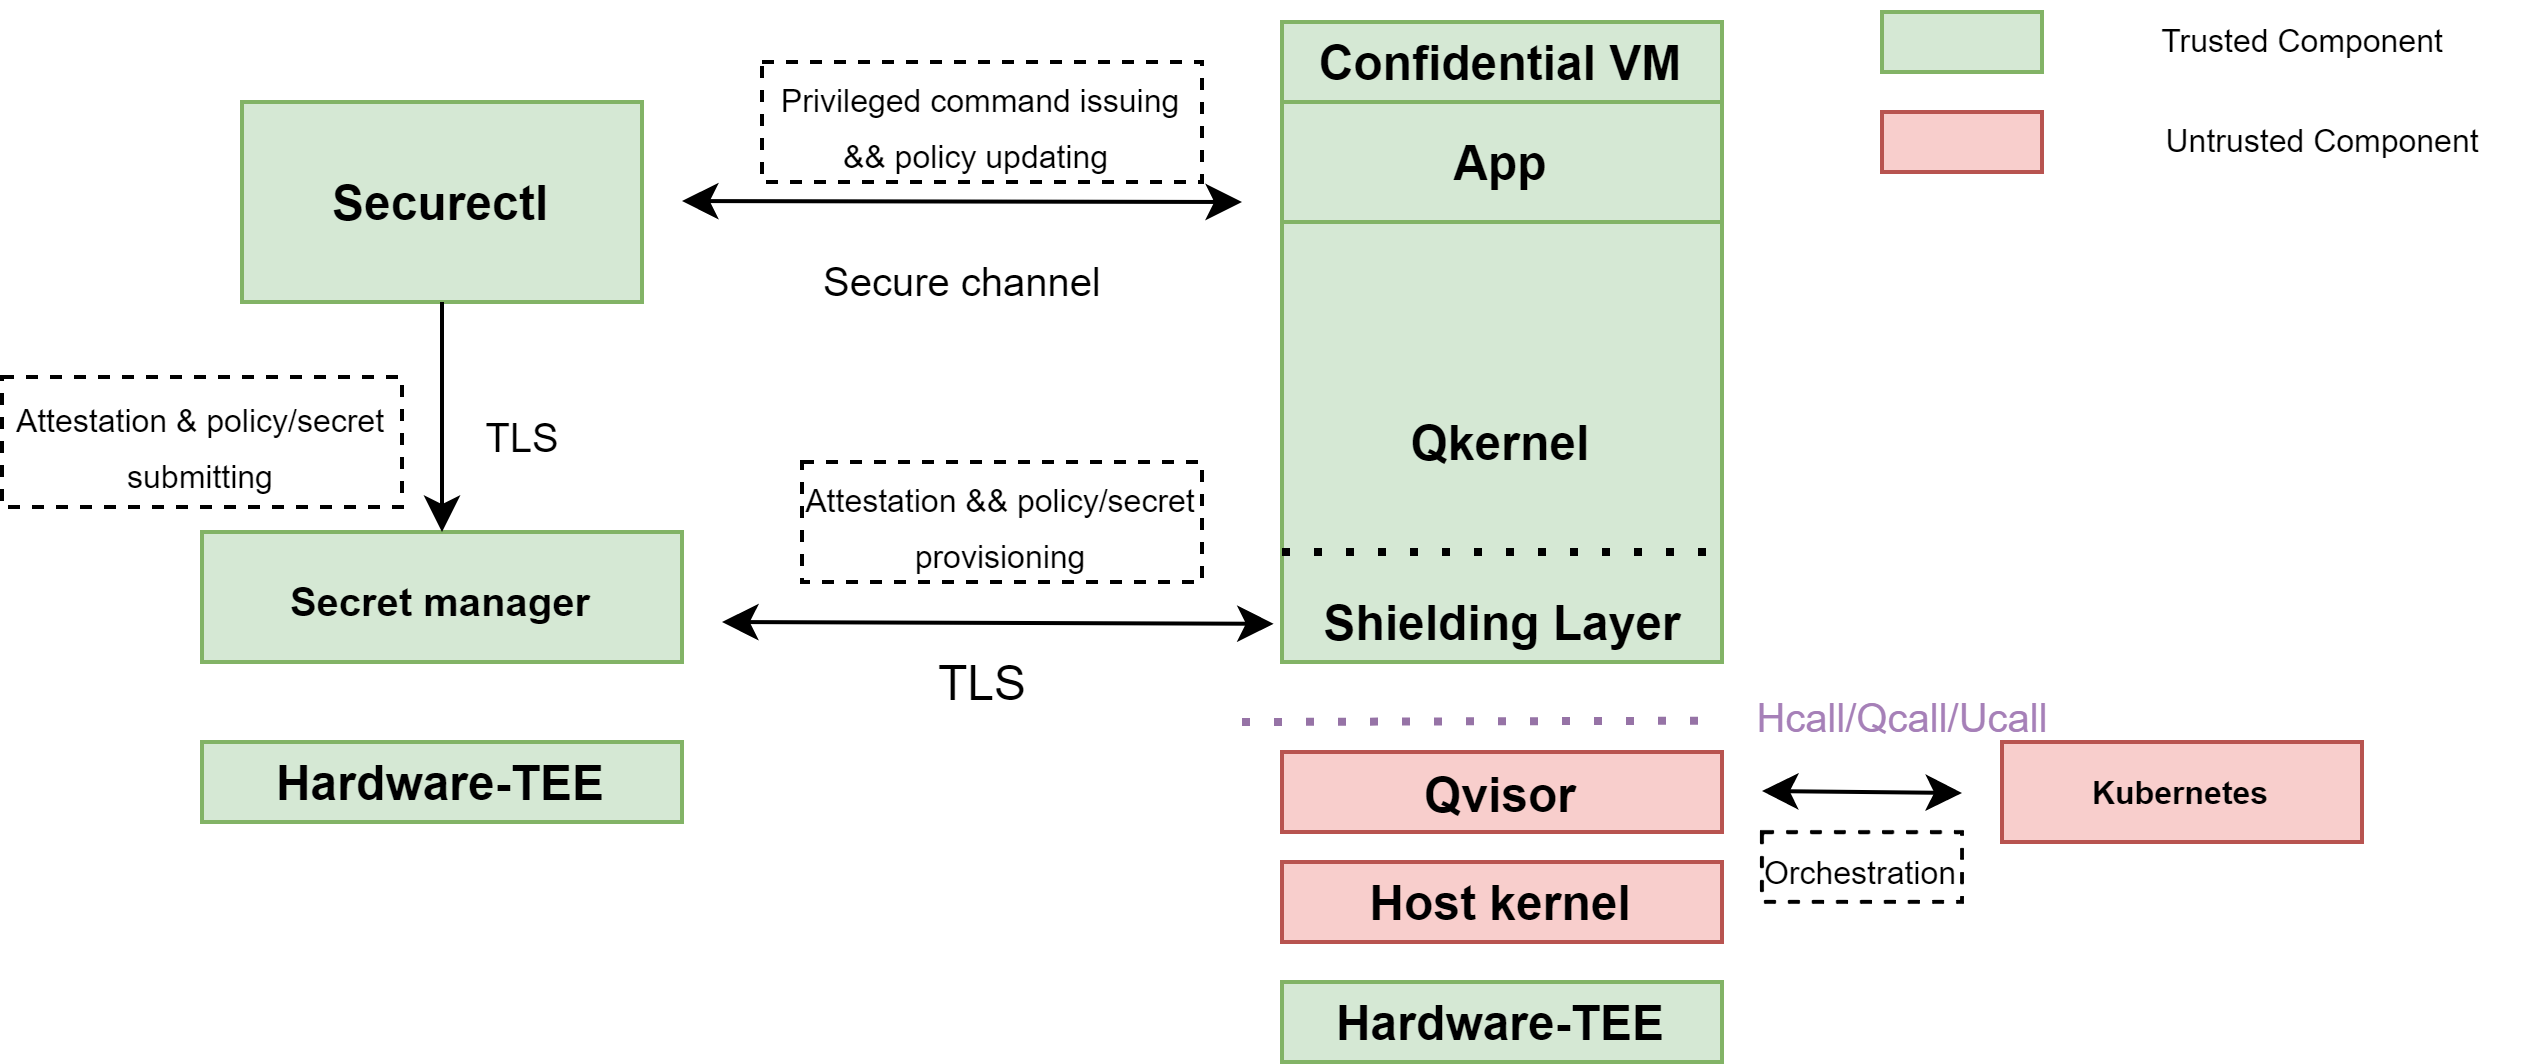
\includegraphics[width=0.8\textwidth]{images/genaral_architechture.png}
    \caption[General Architecture]{General Architecture. The green components in the figure are trusted ,and the red components are not trusted.}
    \label{fig:genaral_architechture}
\end{figure}


On the application owner's side, we introduce Securectl, which establishes a secure channel between the application owner and the enclave. The tool runs in an environment trusted by the application owner and provides an interface to communicate 
with the application and control the shield. The secret manager manages the application's secrets and runs in the cloud, protected by a secure virtual machine. The application owner can authenticate the secret manager using the remote attestation 
mechanism and then upload the secrets through a secure channel. The secret manager validates the application startup process against the policy uploaded by the application owner and securely sends the secrets to the shield. The shield is responsible 
for secret deployment and ensures that the secret is not compromised while the application runs.

\section{Quark Attestation and Provisioning Infrastructure}
This section presents the Quark attestation and provisioning infrastructure, which is designed to facilitate secure application deployment and provides a means for applications to obtain attestation reports at runtime. In particular, it offers mitigation for the following three security issues identified in the security analysis:

Untrusted Kubernetes and Quark-shim manage and deploy applications' secrets.
Corrupted application binaries may be loaded during the application build process.
Lack of measurement of Qkernel command line parameters.

\subsection{Overview}
\begin{figure}[H]
    \centering
    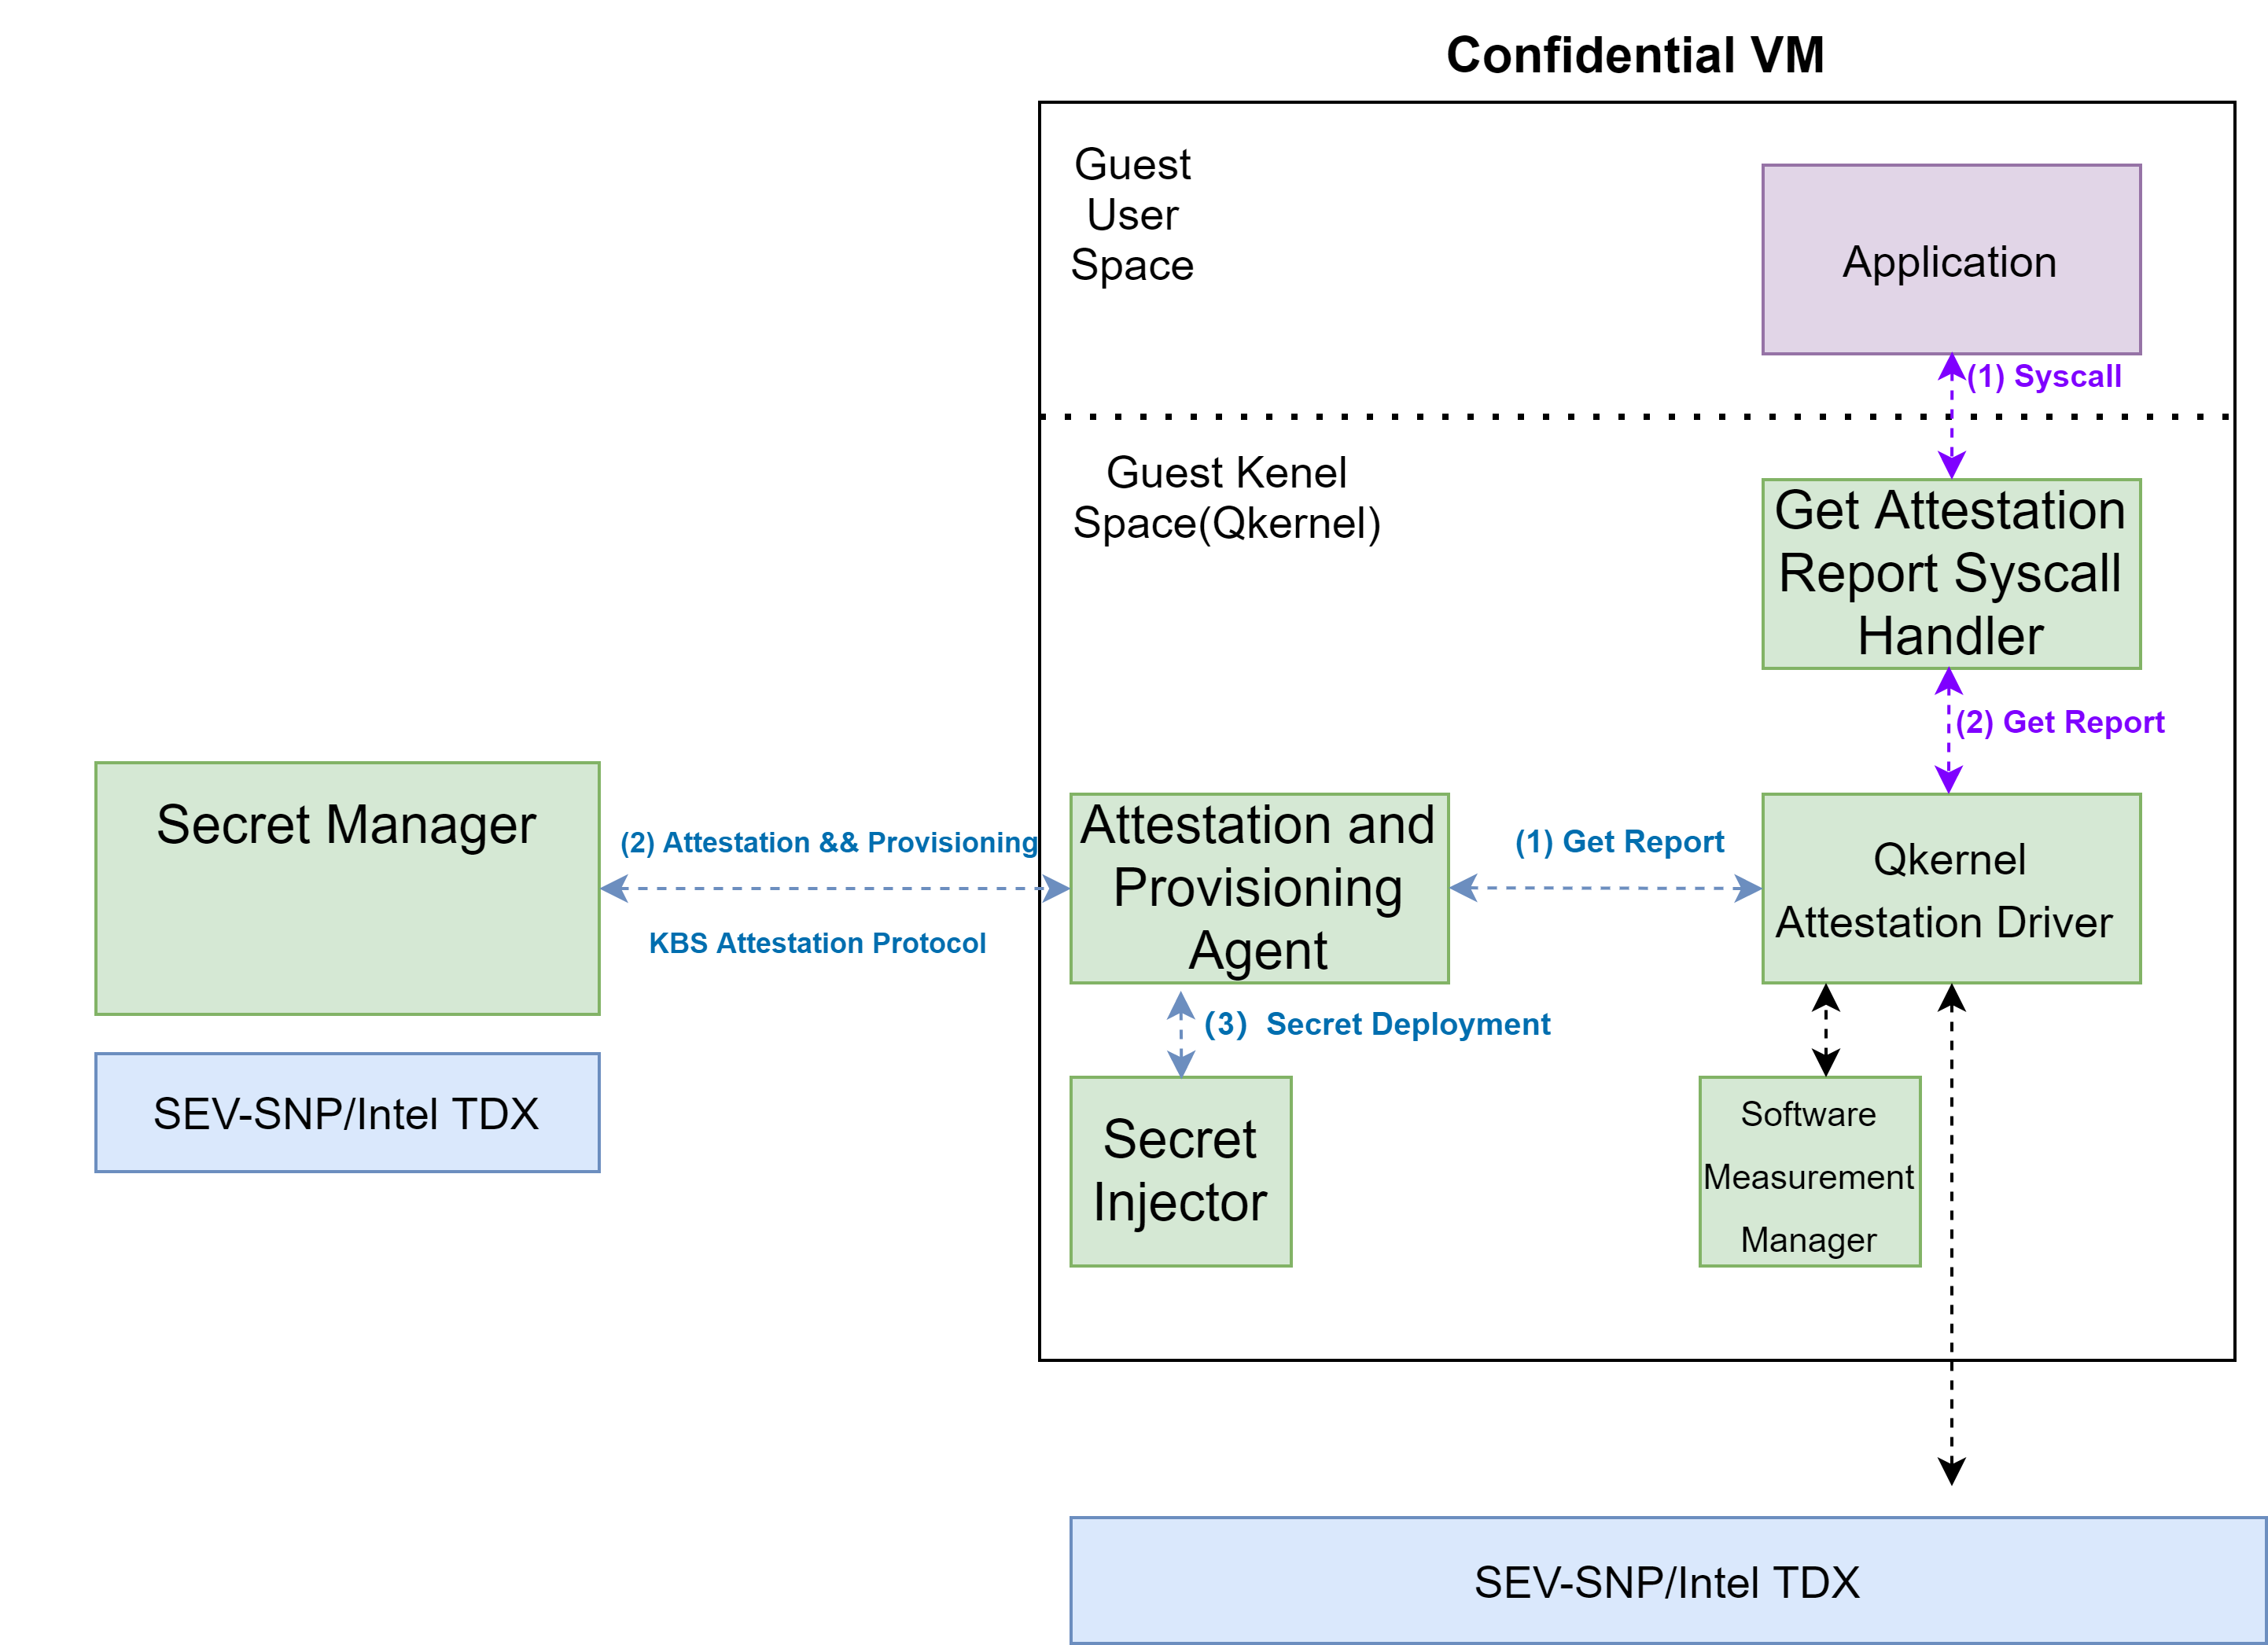
\includegraphics[width=0.8\textwidth]{images/Qkernel_attestation_infrastructurc.png}
    \caption[Quark Attestation and Provisioning Infrastructure]{Quark Attestation and Provisioning Infrastructure}
    \label{fig:Qkernel_attestation_infrastructurc}
\end{figure}

The management and deployment of application secrets are delegated from Kubernetes to the Quark attestation and provisioning infrastructure, as illustrated in Figure~\ref{fig:Qkernel_attestation_infrastructurc}. The infrastructure comprises two 
parts- the secret manager and several components in the enclave shielding layer. These components include the remote attestation and provisioning agent, the secret injector, the Qkernel attestation driver, and the software measurement manager.

The secret manager is responsible for managing and provisioning secrets to the enclave. It runs in a cloud-based trusted execution environment. This guarantees the confidentiality of its managed secrets. The application owner validates the secret 
manager before securely uploading secrets to it. The secrets include the shielding layer's policy, the application's startup parameters, environment variables, and files. The cluster administrator deploys applications. The software measurement 
manager will measure the application binaries and Qkernel startup parameters to ensure correct deployment. The results are sent to the secret manager as part of the enclave's attestation report for integrity check. The report is generated by TEE 
hardware with the help of the Qkernel attestation driver.

During remote attestation and provisioning, the remote attestation and provisioning agent prove its identity to the secret manager and retrieves secrets. This process is done following the KBS attestation protocol. The shielding layer's components 
are then initialized with the policy, and application-related secrets are deployed to the application process by the secret injector. Specifically, the application startup parameters and environment variables are inserted into the stack of the 
application process. For file-type secrets, the injector keeps them in enclave memory as the host is untrusted. To make these file type secrets accessible to the application, the injector creates a subfile system for these secrets using Qkernel's 
virtual file system interface. The file system is mounted in the /secret directory, and the application can access these secrets the same way as any other files in the host rootfs. The difference is that access to these secrets is redirected to the shielding layer instead of the host. In this way, we offload the secret management and deployment from Kubernetes.

Finally, the infrastructure allows applications to obtain attestation reports at runtime through the guest system call interface. For more information, please refer to Section XX.

\subsection{Secret Uploading}

\begin{figure}[H]
    \centering
    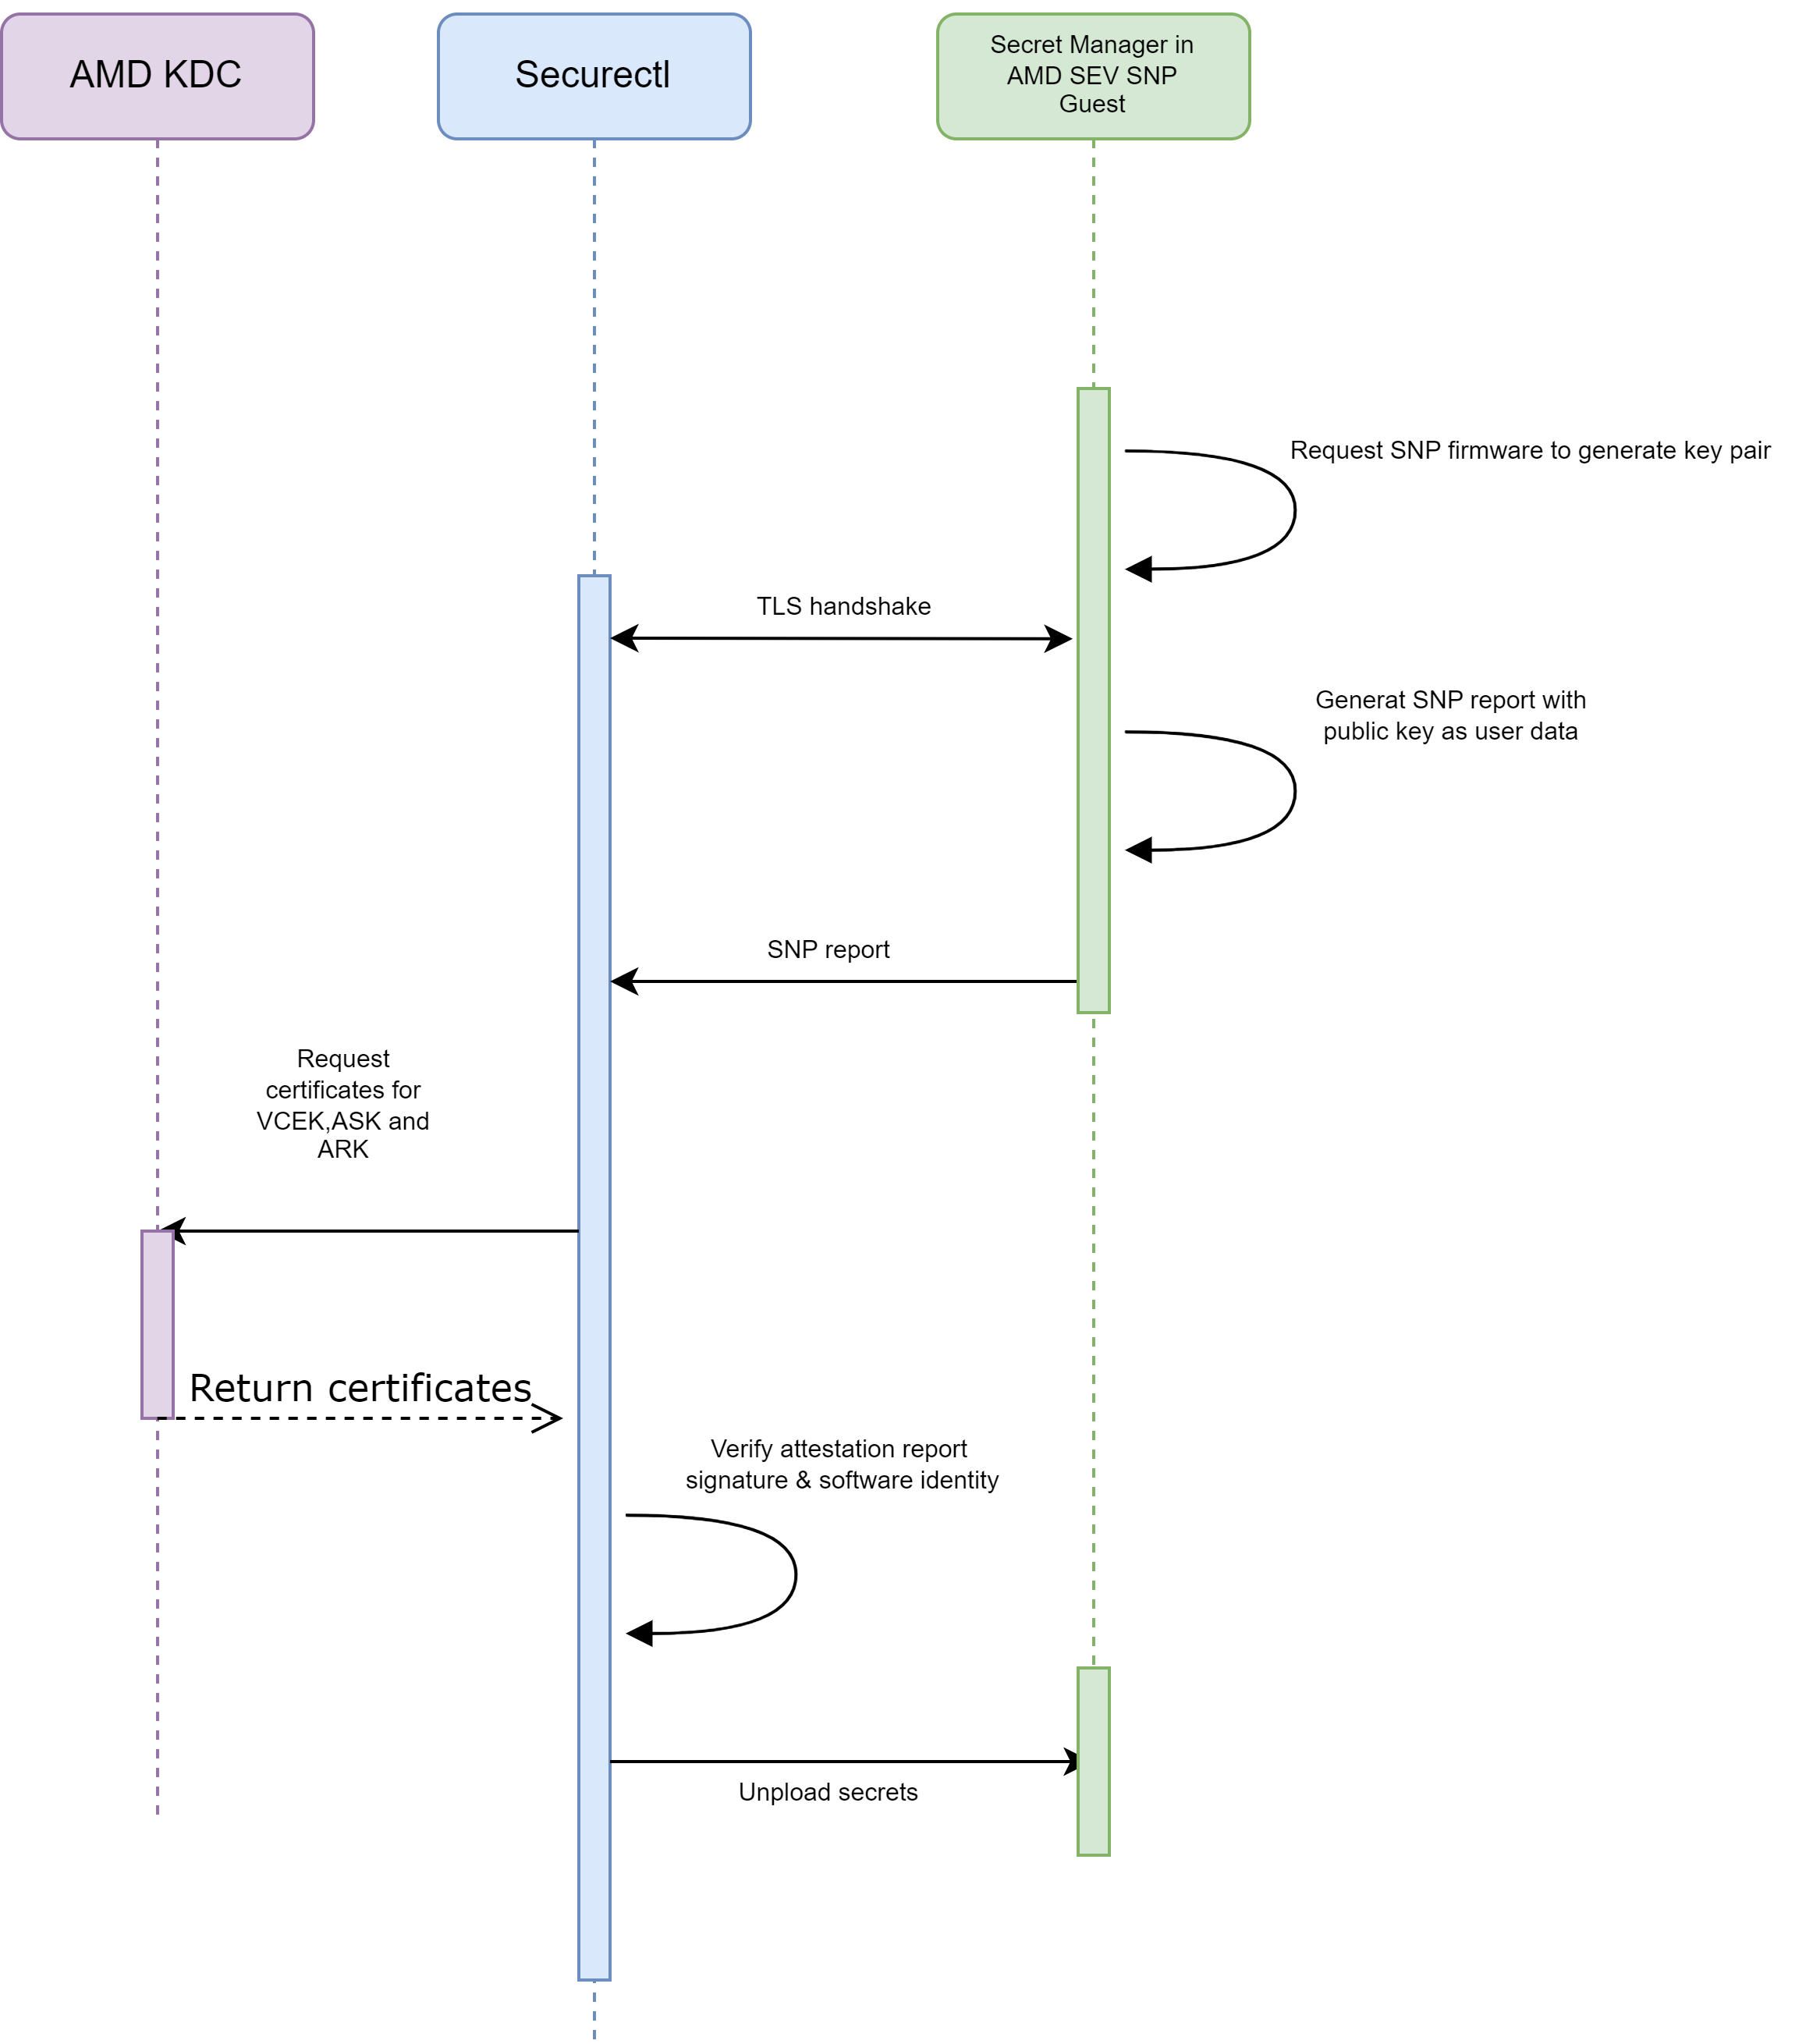
\includegraphics[width=0.8\textwidth]{images/upload_secret.png}
    \caption[Secret Uploading Workflow]{Secret Uploading Workflow. Note that in the figure, the application owner uses Securectl to attest secret manager and upload secrets.}
    \label{fig:upload_secret}
\end{figure}

The process of uploading secrets to the secret manager requires two steps to be taken by the application owner. Firstly, the application owner needs to attest the secret manager. Secondly, a secure channel must be established for the secret uploading.
This process is illustrated in Figure~\ref{fig:upload_secret}. We assume the secret manager is running in the AMD SEV SNP~\cite*{SEV_SNP_white_book}. Initially, 
the secret manager requests SNP to generate a key pair for the TLS connection. The private key of this pair is then stored in the secret manager's memory, which is protected by the TEE.
Since the key pair can only be used by the secret manager, it can be considered as an identifier for the secure channel. To bind the secret manager to the identifier of the secure channel,
the hash of the public key is added to the attestation report of the secret manager. Upon receiving the report, the application owner requests a certificate chain from the AMD KDC using 
the CHIP\_ID and TSB parameters in the report~\cite*{snp_kdc}. The certificate chain is then used by the application owner to verify the signature of the report. Then using the information in the report,
the application owner can ensure that the remote secret manager is genuine and that the hash of the public key used to establish the TLS matches the hash of the public key in the report. 
By fulfilling these steps, the application owner can determines that the entity on the other side of the secure channel is the intended secret manager. Thus, the channel can 
safely be leveraged for the secrets uploading.

\subsection{Secure Application Deployment}

The objective of secure application deployment is to ensure the confidentiality and integrity of an application's sensitive data and the shielding layer's policy. To achieve this goal, a new deployment mechanism is proposed to offload secrets 
management and deployment from Kubernetes, as illustrated in Figure~\ref{fig:attestation_provisioning}.

The cluster operator still uses YAML to deploy applications but without including any secrets. Instead, the application secrets and the policy of the shielding layer are uploaded to the secret manager. The cluster operator only needs to provide the 
IP address of the secret manager and secrets'URL in the YAML. This IP address is used by the remote attestation and provisioning agent to establish a connection with the secret manager during the application process creation, while the URLs are 
employed by the agent to request secrets via the HTTP GET method.

\begin{figure}[H]
    \centering
    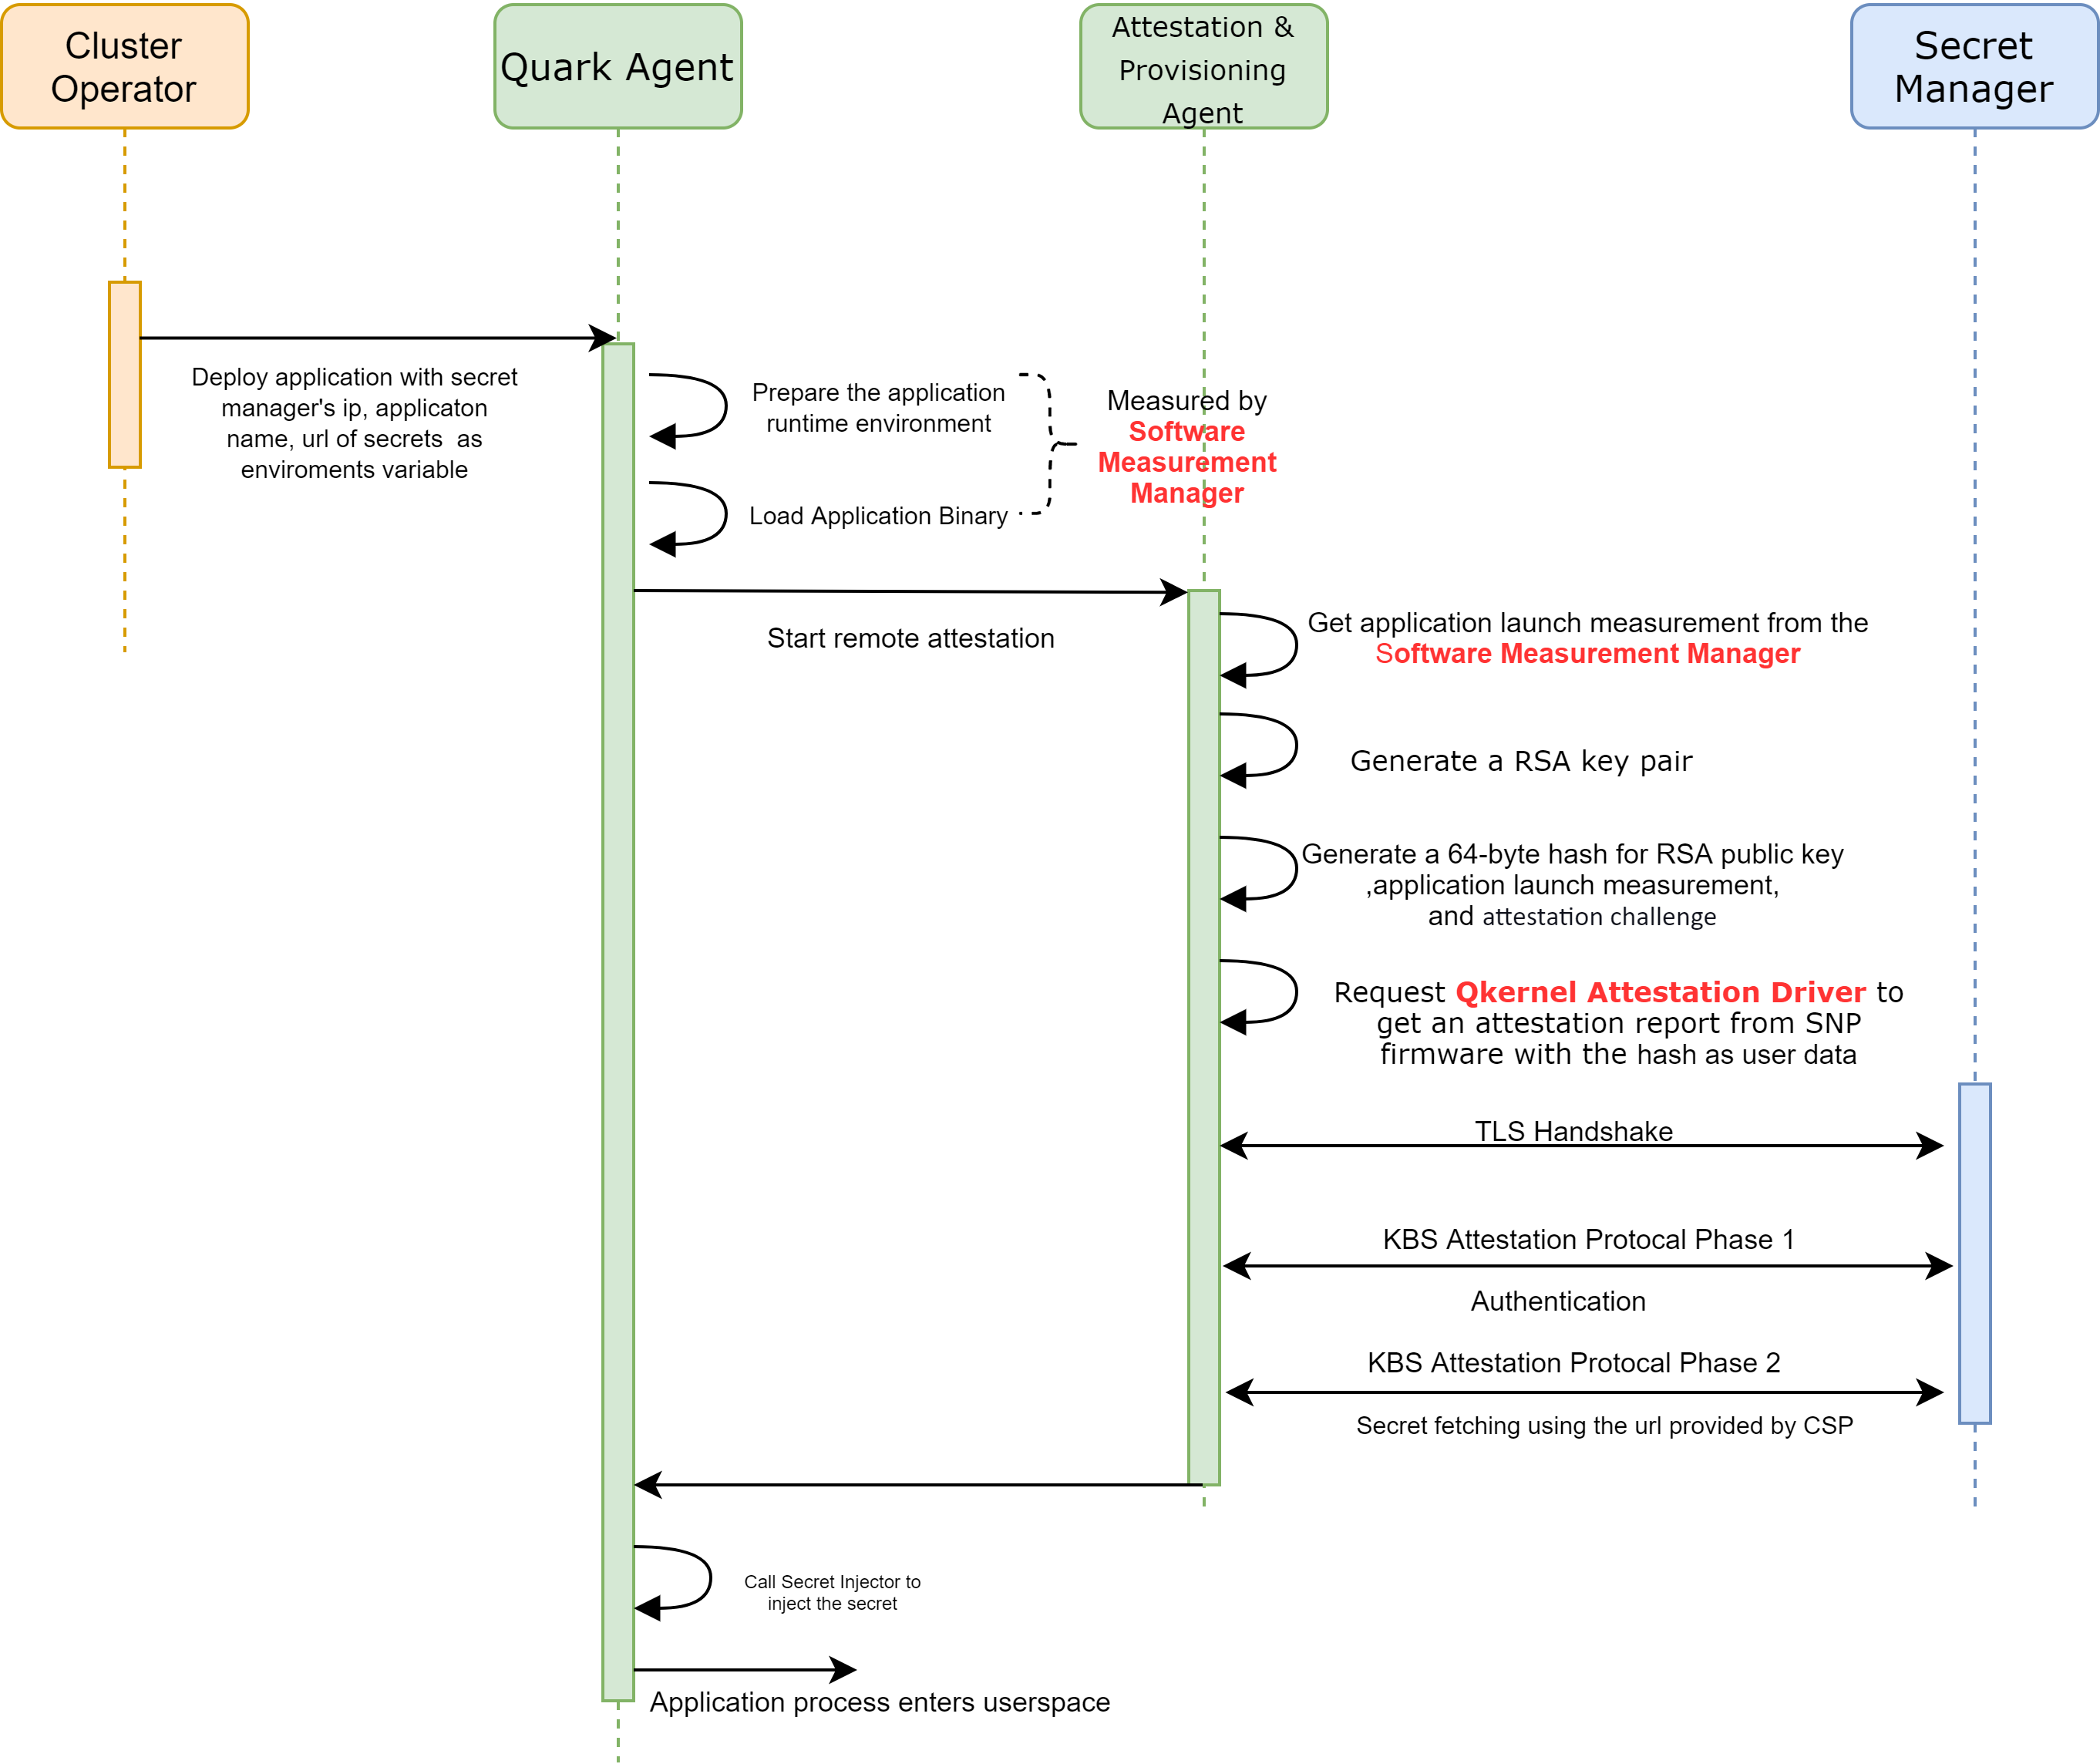
\includegraphics[width=0.8\textwidth]{images/attestation_provisioning.png}
    \caption[Secure Application Deployment Workflow]{Secure Application Deployment. The green components are running in the enclave. The cluster operator is not trusted. The Secret Manager is responsible for managing the secrets as a relying party, attesting  enclave, and provisioning the secrets.}
    \label{fig:attestation_provisioning}
\end{figure}

Upon receiving an application creation request, the quark agent located in the enclave creates the application process based on a process specification. This involves loading the application binaries from the host machine, setting up the file 
system for the application process, etc. To ensure the integrity of the loaded binaries, the software measurement manager extends the loaded binaries with a hash called the enclave start measurement, through which the loaded binaries are bound to 
the enclave start hash. Note that this measurement is constructed at the enclave start, which also includes a measurement of the Qkernel command-line arguments.

\begin{figure}[H]
    \centering
    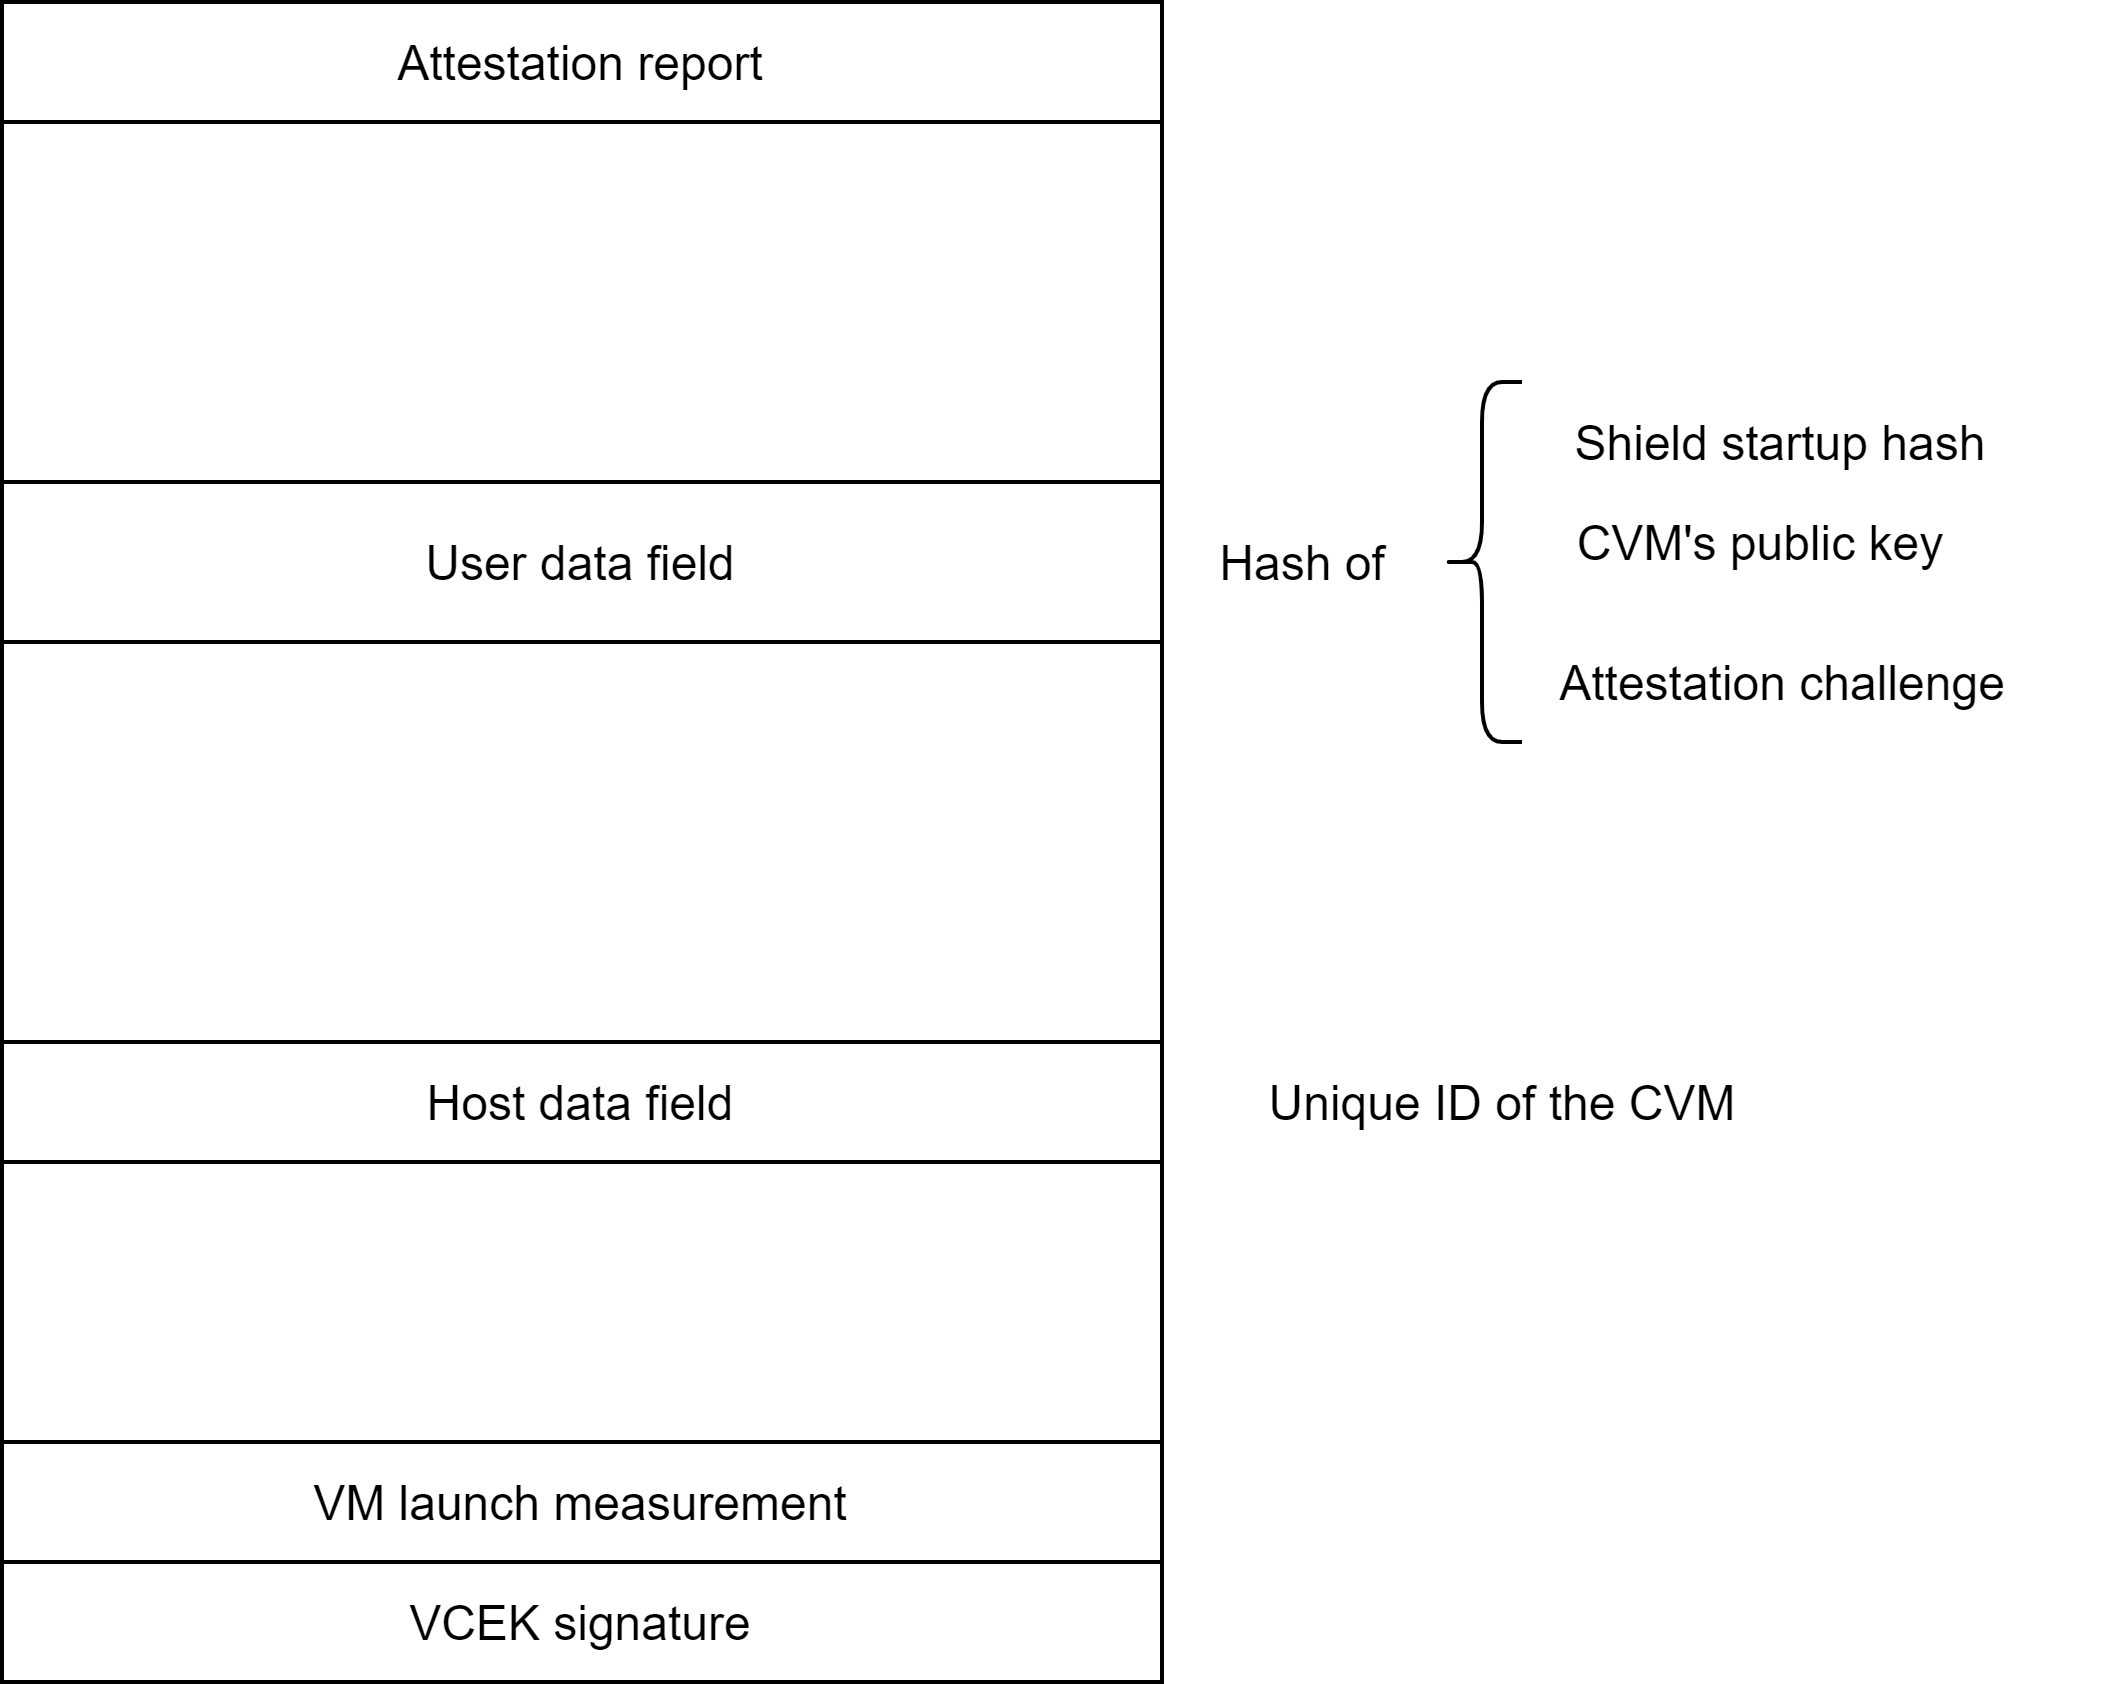
\includegraphics[width=0.8\textwidth]{images/attestation_report_format.png}
    \caption[SNP attestation report]{SNP attestation report.}
    \label{fig:attestation_report_format}
\end{figure}

Subsequently, the remote attestation and provisioning agent requests the Qkernel attestation driver to generate an attestation report. Depending on the type of TEE, the driver will generate a different attestation report. Assuming the enclave runs 
in AMD SNP, the driver will request the SNP firmware to generate the attestation report. Then, the attestation and provisioning agent will connect to the secret manager using the IP address in the YAML and use this report to prove the enclave's 
identity and get secrets from the secret manager following the KBS attestation protocol. The attestation report is shown in Figure 6. It is protected with the VCEK signature and contains:
\begin{itemize}
    \item SNP firmware's measurements for the VM boot process
    \item Tamper-resistant 64-byte user-defined data.
    \item Host data.
    \item VCEK signature.
    \item Others
\end{itemize}


The secret manager verifies the report's signature using the certificate chain required fro AMD KDC~\cite*{snp_kdc}. By examining the virtual machine boot process measurements, the secret manager can confirm that the enclave is using the correct Qkernel binary. 
Since Qkernel is loaded into the enclave memory using SNP\_LAUNCH\_UPDATE~\cite*{snp_firmware} during virtual boot by Qvisor, snp firmware also measures the Qkernel binary. Notably, the code of the shielding layer is part of the Qkernel binary.

The user-defined data in the attestation report is a hash, including the enclave startup measurement and a hash of the TEE-generated public key. The enclave startup measurement is created by the software manager and incorporates all the sensitive 
data that the enclave loads from the host after the enclave starts until the application is loaded. This includes the Qkernel command line parameters, the binaries loaded during the application startup, and the secret manager's public key. By 
comparing the enclave startup measurement with the reference hash provided by the application owner, the secret manager can verify that the enclave is appropriately configured and that only legitimate binaries are loaded.

To establish a secure channel for secrets provisioning, the KBS attestation protocol~\cite*{kbs_Attestation_protocol} necessitates that the enclave generates an asymmetric key pair from TEE. During the authentication phase of the protocol, the public key is sent to the secret 
manager with an attestation report. In the second phase, the secret manager uses this public key to encrypt the secret requested by the enclave. By incorporating the public key hash in the enclave's attestation report, the secret manager can 
determine that the public key belongs to the enclave, and only the enclave can decrypt the encrypted secret.

To prevent an attacker from hijacking the secret manager's address and impersonating the secret manager, the remote attestation and provisioning agent use the secret manager's public key to verify the secret manager's identity during the TLS 
handshake. Note that Kubernetes mount the public key of the secret manager as a file on the application's rootfs. To this end, an attacker can provide a bogus public key to the remote attestation and provisioning agent to trick it into establishing 
a connection with the fake secret manager. To address this, the remote attestation and provisioning agent reads the secret manager's public key into the guest's memory and add the key's measurements to the enclave startup measurement. This way, 
the secret manager can verify that the remote attestation and provisioning agent uses the correct public key. When an attacker presents the remote attestation and provisioning agent with a fake secret manager's public key, the TLS handshake fails 
due to a mismatch between the public key and the certificate of the real secret manager. Even if the TLS is established, the real secret manager will reject the authentication request from the agent because the enclave startup measurement does not 
match the reference hash.

Since all enclaves use a standard Qkernel binary and applications are created from standard images, the attestation evidence cannot uniquely identify an enclave. Instead, the evidence only certifies that the attester is an enclave running in a 
TEE with the correctly loaded application. Hence, If the secret manager identifies the enclave only based on the attestation evidence, an enclave belonging to one stakeholder could steal the secrets of another stakeholder. To circumvent this, 
the application owner should assign a unique ID to each enclave. This ID should be added to the host data field in the attestation report by Qvisor during enclave setup using SNP\_LAUNCH\_FINISH~\cite*{snp_firmware}. This field is immutable after launching the enclave, 
so the ID is bound to the enclave's attestation evidence. When the secret manager receives an enclave's attestation report, it can use this ID to determine its identity. In the authentication phase of the KBS attestation protocol, the secret 
manager assigns a cookie identifier to an enclave's HTTP request, binding the enclave's ID and attestation result to the cookie identifier. In the second phase, the secret manager maps the cookie identifier in the attester's resource request message 
to its attestation result and the enclave's ID. The secret manager uses this information and the data owner-defined policy to determine whether to grant access to a particular secret to the attester. 

The attester's resource request URL has the following format: <repository>/<type>/<tag>, where <repository> is similar to the concept of container image repository, <type> is used to distinguish between different resource types, and <tag> is used 
to distinguish between different versions of a resource. In the secret manager, each user has a unique repository. The secret manager allows users to specify which enclaves with which IDs can access this repository. In this way, we effectively avoid 
cross-leakage of secrets between different stakeholders.

\subsection{Application Runtime Attestation Service}

An application may need to authenticate itself to a remote end at runtime. Quark attestation and provisioning infrastructure enable applications to obtain attestation reports through the guest system call interface. 
Depending on the application's needs, one of three report formats can be obtained: an attestation report generated by the TEE hardware and two software attestation reports created by the shielding layer. The latter contains:
\begin{itemize}
    \item Enclave start-up measurement.
    \item Enclave ID.
    \item Signature.
    \item Sixty-four bytes of application-specified data.
  \end{itemize}

The application can choose to sign the software report with a key issued by the secret manager or by a key it provided. The secret manager key is sent to the enclave along with the application's secret during the creation of the application process. 
Software reports offer additional possibilities for how the application proves its identity to the remote end. In other words, the remote end can verify the report without the assistance of the hardware provider. Upon verification of the report, 
the remote end can ensure that the application is as expected by using the enclave start-up measurement. Additionally, application-defined data in a software report is tamper-proof, similar to user data in SNP reports. As previously discussed, the 
enclave ID guarantees that the remote end can determine the application's identity, which prevents secret cross-leakage.



\section{Enclave Runtime Measurement}
Enclave runtime measurements are crucial due to the security analysis findings discussed in Chapter~\ref{sec:security_analyse}. Qkernel command line parameters, the application binary, and shared libraries are loaded from the host. Thus, an attacker can modify them 
to breach the enclave's confidentiality. However, AMD SEV SVP does not facilitate enclave runtime measurements~\cite*{snp_firmware}, and INTEL TDX only allocates four registers for this purpose~\cite*{Intel_tdx_whitepaper}. Consequently, we provide a software measurement manager in the shielding 
layer to measure the data loaded from the host while the enclave is running. The software measurement manager obtains the following important measurements by measuring these data.

\textbf{Enclave startup measurement.} This value refers to the measures of host-loaded data from the enclave starting until the enclave finishes loading the application binaries. To config the application's execution environment, the enclave may have to 
execute multiple binaries first. For example, Nginx startup necessitates the enclave to execute a docker-entry.sh shell script\cite*{nginx}. The shell script then executes several Linux commands. Each is a binary. Therefore, the enclave startup measurement may 
comprise binaries, shared libraries, Qkernel boot parameters, and the secret manager's public key. The attestation and provisioning agent include this measurement in the attestation report, which is conveyed to the secret manager. The secret manager 
compares the measurement to the reference value provided by the enclave owner to ensure that the enclave is genuine.

\textbf{Application startup measurement.} This value records the measure of all binaries and shared libraries loaded from the time the enclave receives the application creation request to the point when the enclave completes loading the application binaries. 
This measurement is a subset of the enclave startup measurement and is stored in the enclave memory. It serves as a reference hash with the application restart measurement.

\textbf{Measurement of binaries at application runtime.} The application process loads its shared libraries after it enters the user space. Moreover, the enclave creates a process and loads the corresponding binary from the host when a user initiates a 
command to the application. The software measurement manager measures the loaded binaries or shared libraries to prevent an attacker from serving compromised binary to the enclave. However, unlike the enclave startup measurement, which is forwarded 
to the secret manager, the runtime measurements are verified by the software manager. The shielding layer's policy holds reference measurements for the runtime binaries, as shown in Figure~\ref{fig:measurement}. In this case, the software measurement manager measures 
the binaries and compares the result with reference values from the policy. If the two values differ, the enclave will panic. This ensures that during application runtime, the correct binaries are loaded.

\begin{figure}[H]
    \centering
    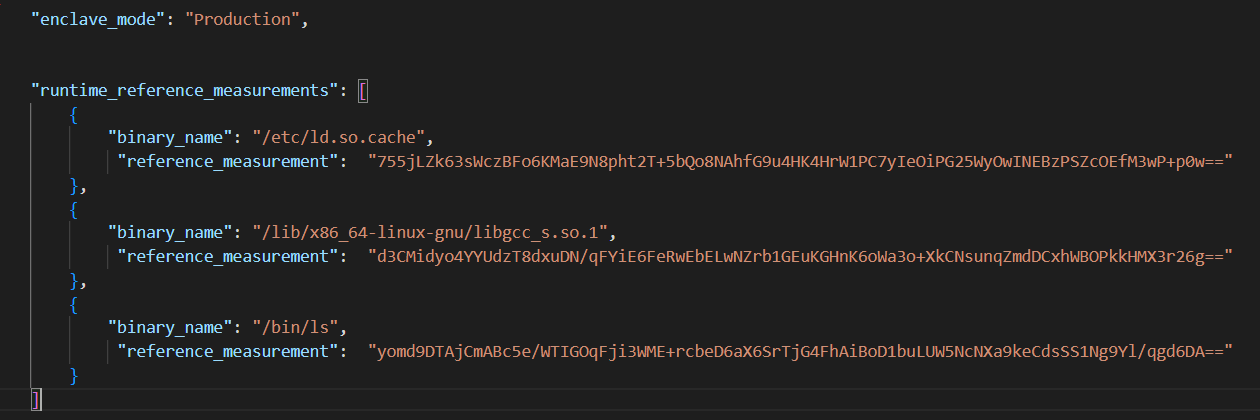
\includegraphics[width=0.8\textwidth]{images/measurement.png}
    \caption[Reference Value in Shielding Layer's Policy for Runtime Binary Measurement]{Reference Value in Shielding Layer's Policy for Runtime Binary Measurement}
    \label{fig:measurement}
\end{figure}

\textbf{The application restart measurement.} In the event of an application crash where the enclave is not exited, Kubernetes will attempt to restart the application within the enclave. The enclave will therefore recreate the application process, load the relevant 
binaries, and inject secrets stored in the enclave's memory. An attacker may exploit this situation by injecting malicious code into the enclave to retrieve secrets, thereby breaching the enclave's confidentiality. One potential solution is to 
measure the loaded binaries or shared libraries during the application restart and send the result to the secret manager for verification. However, this approach is costly as it involves generating an attestation report and communicating with the 
secret manager via the network. Therefore, the software measurement manager stores application startup measurement and uses it as a reference hash for application restart measurement. If the two do not match, the enclave will panic. In doing so, 
the enclave ensures that the binary loaded at restart is identical to the binary loaded during the initial application launch. As the binary's measurements during the first launch are sent to the secret manager for integrity checking, comparing the 
two hashes guarantees the integrity of the loaded binary during application restart.

Regarding obtaining the reference values for enclave startup measurement and measurement of individual binaries loaded at application runtime, we implemented a developer mode for the enclave. When running in developer mode, the enclave prints the 
enclave and application runtime measurements for each binary and shared library to the Qkernel log on the host. The application owner should operate the enclave in a trusted environment to obtain these reference values.


\section{New Pattern for EXEC Requests}

\subsection{Overview}



\begin{figure}[H]
    \centering
    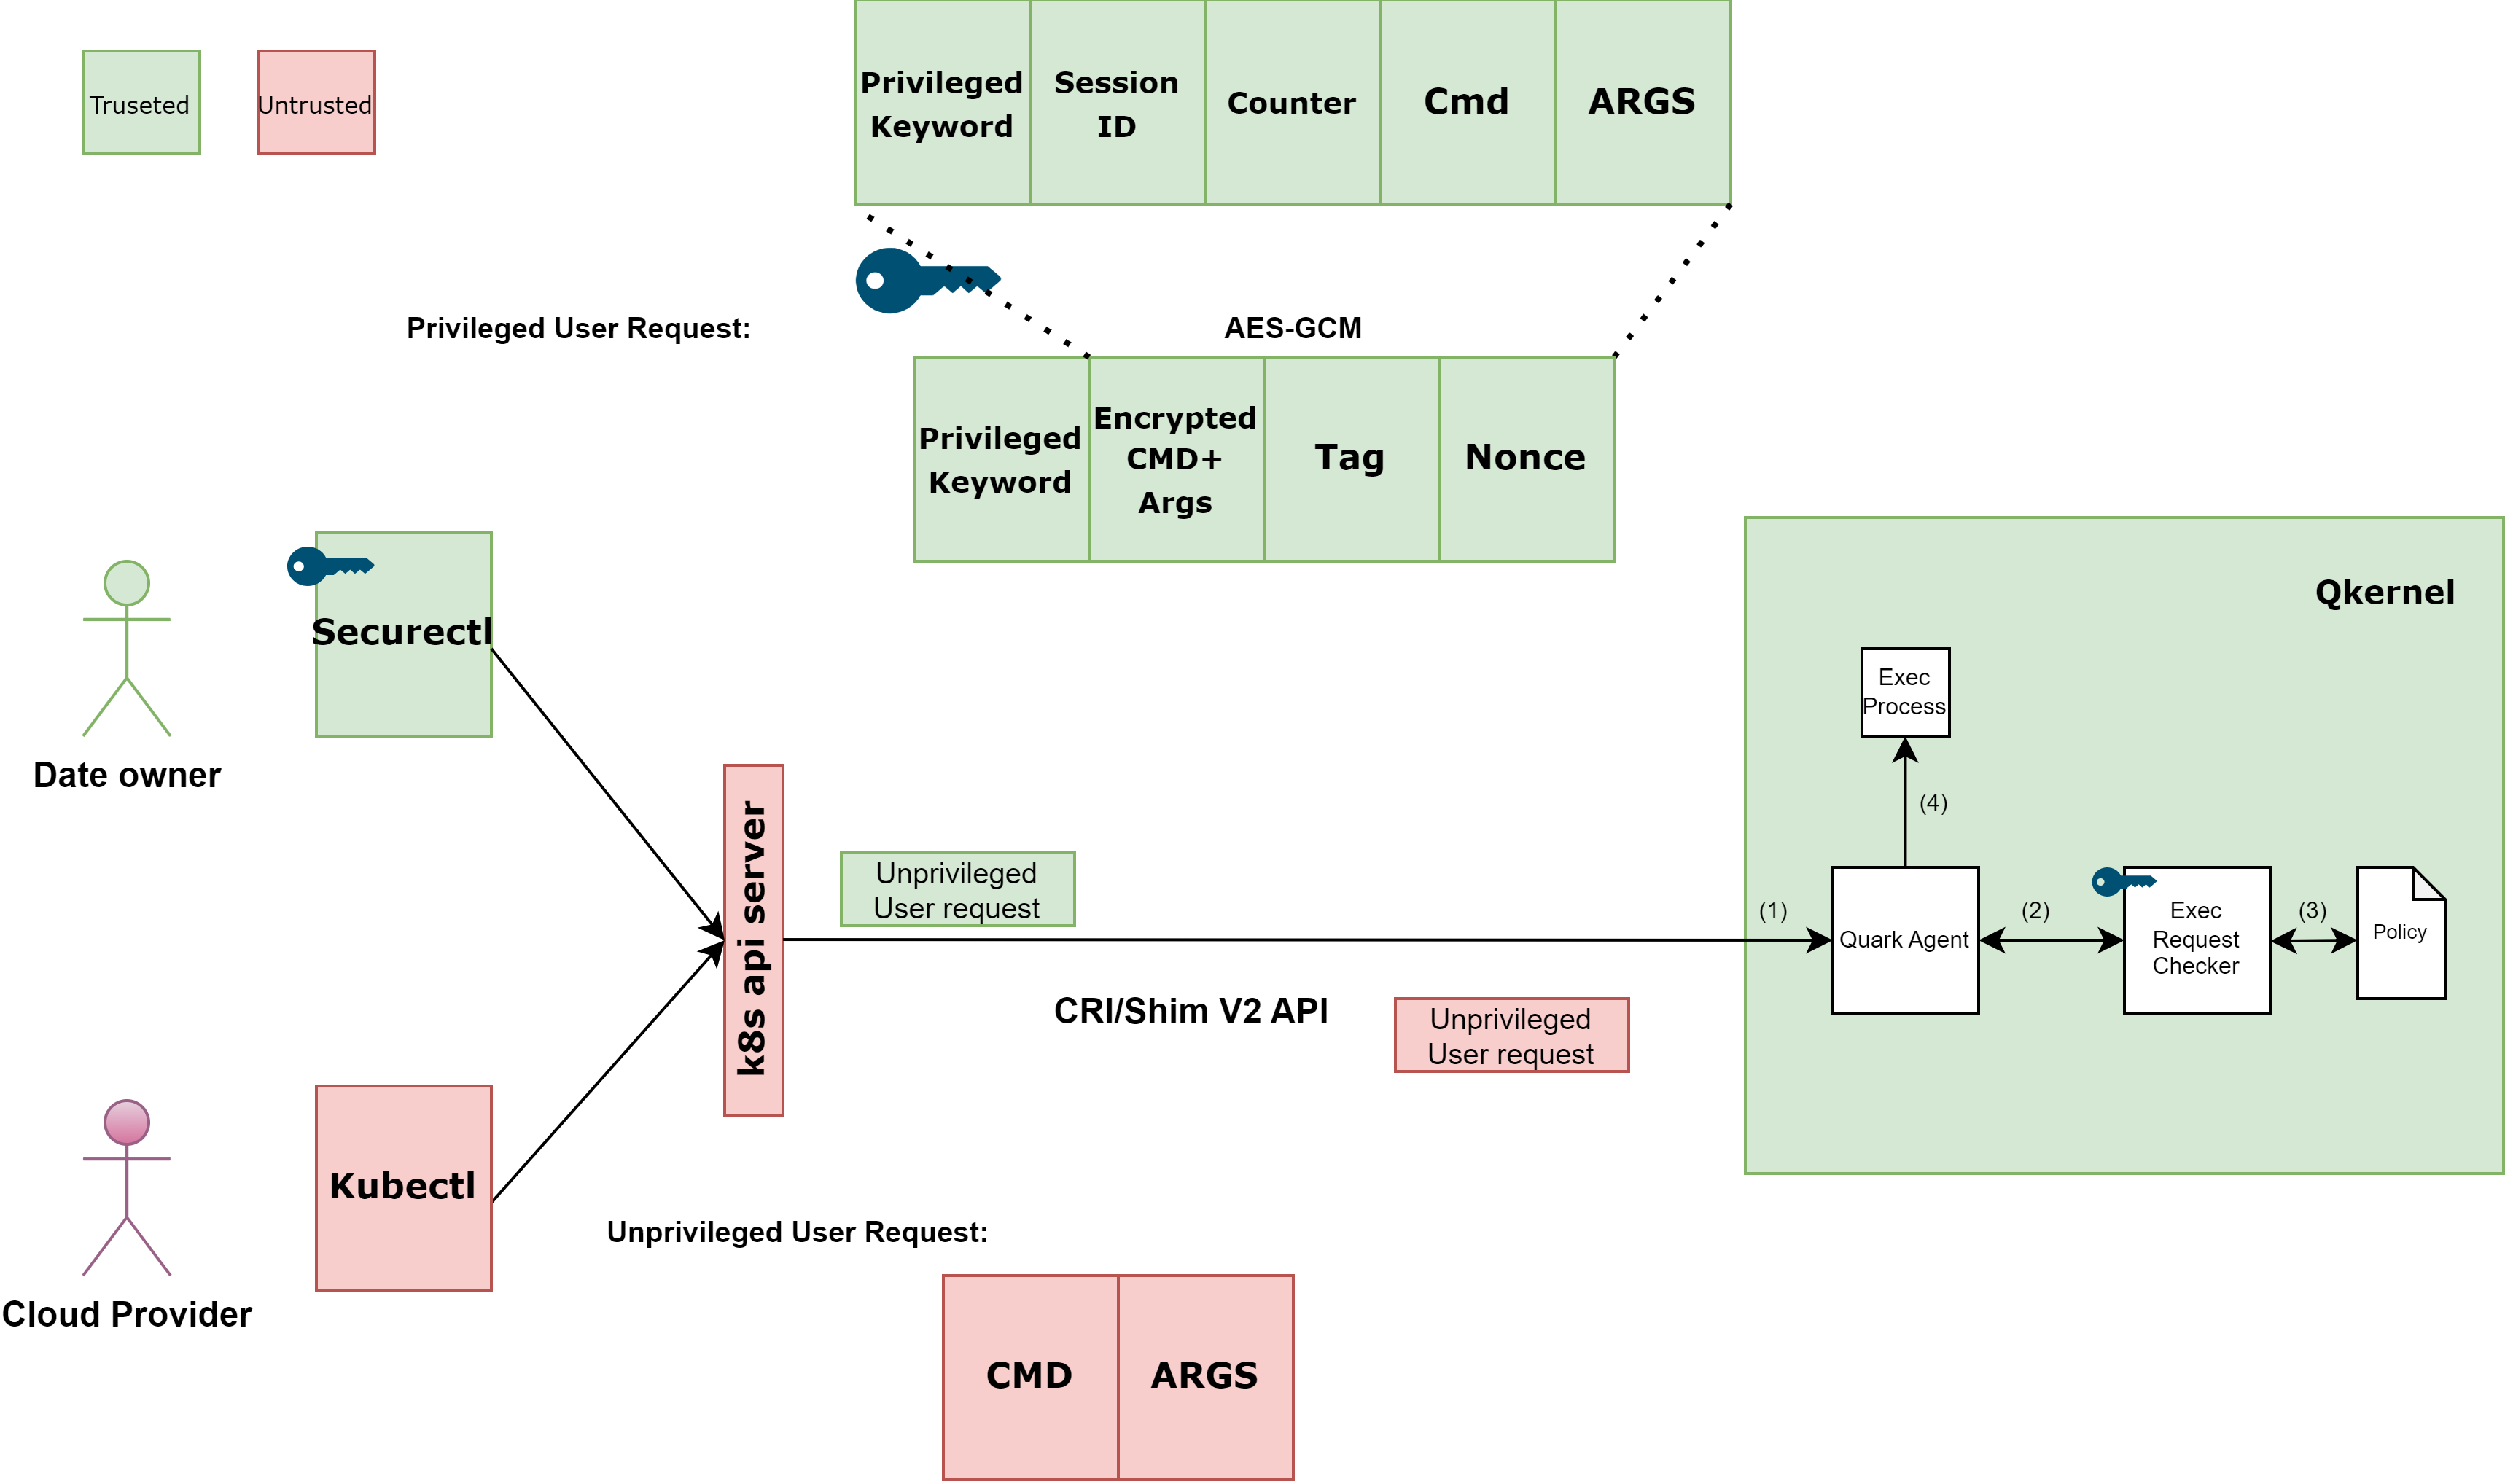
\includegraphics[width=0.8\textwidth]{images/new_pattern_of_exec.png}
    \caption[New Pattern for EXEC Requests]{New Pattern for EXEC Requests}
    \label{fig:new_pattern_of_exec}
\end{figure}


Any user can send an EXEC request to an application. As analyzed in Chapter~\ref{sec:security_analyse}, when a user issues a command to an application or allocates a terminal, Kubernetes will send an EXEC request to the Quark agent located in the enclave. After receiving 
the request, the Quark agent creates a process to execute the command binary (For a terminal allocation request, the command is /bin/bash). Note that the o only difference between issuing a command and allocating a terminal is that the terminal 
keyword is true in the process specification of the exec request for allocating a terminal. Thus, we refer to both issuing a command and allocating a terminal collectively as the EXEC request. Since the Quark agent lacks authentication and access 
control for EXEC requests, an attacker can send arbitrary EXEC requests to an application. Therefore, a new pattern for EXEC requests is proposed, illustrated in Figure~\ref{fig:new_pattern_of_exec}.

The pattern divides EXEC requests into two categories, namely privileged and unprivileged EXEC requests. Privileged EXEC requests are issued by privileged users, i.e., the application owner, while non-privileged requests are issued by untrusted 
entities. An untrusted entity here refers to someone other than the application owner. Privileged and unprivileged users send privileged or unprivileged requests to the enclave using secretctl or kubectl, respectively. Both requests are redirected 
to the enclave through the Kubernetes  API server and the CRI, Shim V2 API interface. Upon receiving the EXEC request, the Quark agent forwards it to the Exec request checker. The Exec request checker will authenticate and access control the request 
according to the enclave policy, as shown in Figure 5. The Quark agent will decide whether to create the EXEC process based on the results returned by the Exec request checker.


\subsection{Protection for Privileged Exec Request}
Since privileged EXEC requests are transmitted through the Kubernetes  component to the enclave, the authenticity, integrity, and confidentiality of the commands and their parameters in requests must be protected. In addition, we must implement a mechanism 
to distinguish between privileged and unprivileged requests. This can be achieved through the frame structure as in Figure~\ref{fig:new_pattern_of_exec} and the use of authenticated encryption operations with associated data, i.e., the Advanced 
Encryption Standard Galois/Counter Mode (AES-GCM)~\ref{aes_gcm}. The frame structure encapsulates the AES-GCM's random number (nonce) for secret decryption, the authentication Tag, the encrypted payload, and the keyword 'Privileged'. Since the Open Container 
Initiative requires that commands and their arguments be passed as a vector of strings, the encrypted payload, nonce, and tag are encoded in base64. The plaintext payload contains the keyword 'Privileged,' the session ID, a counter, the command, 
and its parameters.

AES-GCM~\ref{aes_gcm} ensures the confidentiality, authenticity, and integrity of privileged EXEC requests. Besides, it is easy to deploy as it requires only a shared key. After a successful remote attestation, a key is shared between the application owner and 
the enclave. The application owner can use this key to encrypt privileged commands and their parameters. When the enclave receives a privileged request, the exec request checker can use the key to confirm that the request was generated by a 
privileged user who knows the key (authentication), verify the request's integrity, and decrypt the request.


The keyword "Privileged" is used to distinguish privileged from non-privileged commands. The Kubernetes API requires the user to pass a command, and it's parameters as an array of strings, where the first element is the command and the remaining elements 
are the parameters, e.g. ["cat", "/var/log"]~\cite*{k8s}. Privileged-level commands are passed to the enclave as string arrays through the Kubernetes  API, just like non-privileged-level commands. Thus, the string arrays corresponding to privileged-level commands have 
the following format ["Privileged", "Encrypted cmd + arg," "Tag ","Nonce"]. When the exec request checker receives an EXEC request, it can determine if it is privileged by checking the first element of the command array. Note that the command array 
is part of the EXEC request process specification known as args.


The  monotonic counter and session are designed to prevent reply attacks. Since the privileged Exec requests are transmitted to the enclave by Kubernetes , an attacker can intercept a privileged request and send it continuously to the enclave to 
interfere with its operation. In addition, it can analyze the execution result of an EXEC request. Although the result is encrypted, it may get different results from executing the same command twice. In this case, it may be possible to derive the 
plaintext by analyzing the changes in the ciphertext.   Therefore, we introduce a monotonic counter for privileged-level EXEC requests. This counter is assigned by the enclave to privileged users. When the value of the monotonic counter in an EXEC 
request is smaller than the reference value stored in the enclave, the request is rejected. Since there may be more than one privileged user, it is not easy to share the counter. Therefore, we introduce sessions. In this case, the enclave will 
assign each privileged user a random session id and a unique counter. This id and counter are stored in the enclave and will be sent to a privileged user via a secure channel. The privileged user can use the session id and counter to construct a 
privileged EXEC request. Note that the counter is added by one after each EXEC request.


With the session and counter, we avoid the following two reply attacks. First, the attacker sends a request that belongs to an illegal session, i.e., the session id is not stored by the enclave. Second, the attacker has sent an outdated request to 
the enclave. This means that the counter value in a request is less than the current counter value recorded in the enclave for the requested session ID. In this case, the enclave will refuse to execute it.

\subsection{Session Assignment}

Figure~\ref{fig:session_base_auth} demonstrates how a privileged user gets a session. In the login phase, a privileged user submits a login request using securectl. The login request is a privilege EXEC. However, the payload of the privileged EXEC 
request contains the keyword Login plus a random number instead of a real Linux command. The random number is used to prevent reply attacks. When the request is received and verified by the enclave,  it assigns a session id and a unique counter to 
the privileged user. These two values are stored in the enclave and returned to securectl. The enclave returns these two values via the stdout of the exec process.

\begin{figure}[H]
    \centering
    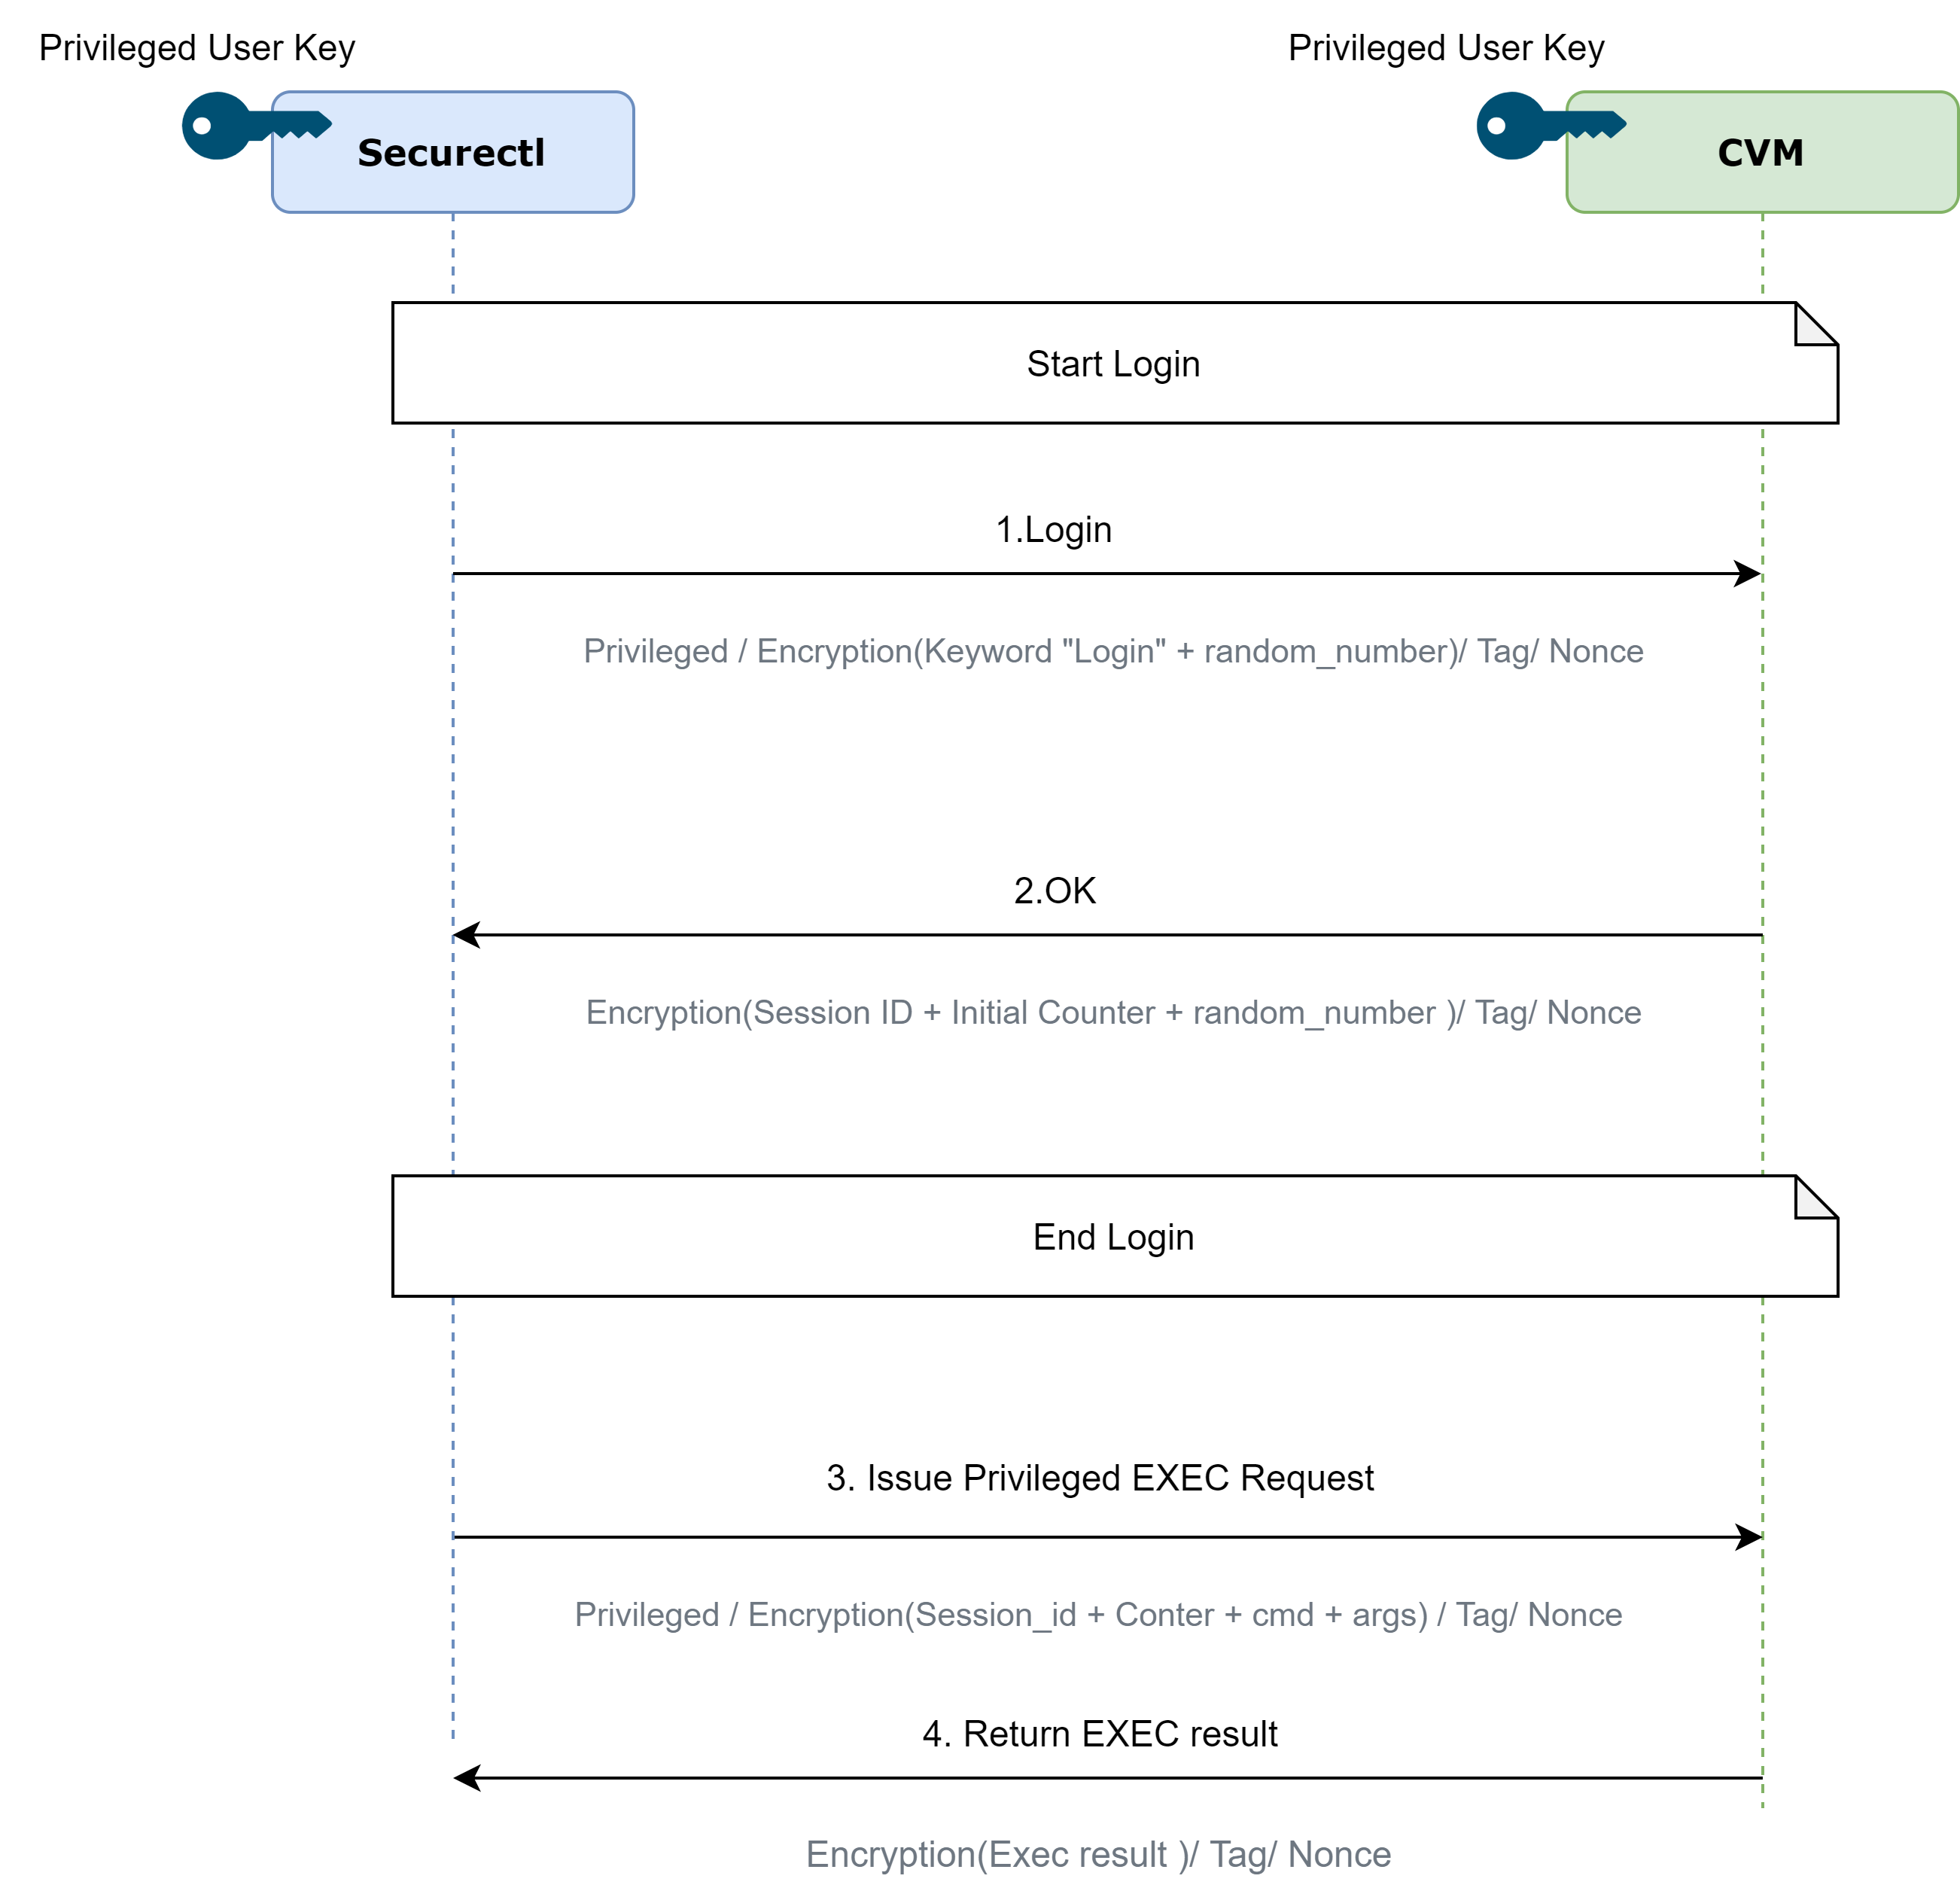
\includegraphics[width=0.8\textwidth]{images/session_base_auth.png}
    \caption[Session Assignment]{Session Assignment}
    \label{fig:session_base_auth}
\end{figure}

When the enclave receives the exec request, it creates a process based on the exec request's process specification. However, the keyword "Login" is not a Linux command. Thus, the enclave replaces the command executed by the exec process with "ls." 
Once the process completes running ls and writes the result to the process's STDOUT, the STDIO shield intercepts the data written to STDOUT and replaces it with the privileged user-assigned session ID and counter. Since the login request is 
privileged, its output is cryptographically protected.



\cleardoublepage

%%% Local Variables:
%%% TeX-master: "diplom"
%%% End:
